% This is "sig-alternate.tex" V2.1 April 2013 
% This file should be compiled with V2.5 of "sig-alternate.cls" May 2012
%
% This example file demonstrates the use of the 'sig-alternate.cls'
% V2.5 LaTeX2e document class file. It is for those submitting
% articles to ACM Conference Proceedings WHO DO NOT WISH TO
% STRICTLY ADHERE TO THE SIGS (PUBS-BOARD-ENDORSED) STYLE.
% The 'sig-alternate.cls' file will produce a similar-looking,
% albeit, 'tighter' paper resulting in, invariably, fewer pages.
%
% ----------------------------------------------------------------------------------------------------------------
% This .tex file (and associated .cls V2.5) produces:
%       1) The Permission Statement
%       2) The Conference (lo cation) Info information
%       3) The Copyright Line with ACM data
%       4) NO page numbers
%
% as against the acm_proc_article-sp.cls file which
% DOES NOT produce 1) thru' 3) above.
%
% Using 'sig-alternate.cls' you have control, however, from within
% the source .tex file, over both the CopyrightYear
% (defaulted to 200X) and the ACM Copyright Data
% (defaulted to X-XXXXX-XX-X/XX/XX).
% e.g.
% \CopyrightYear{2007} will cause 2007 to appear in the copyright line.
% \crdata{0-12345-67-8/90/12} will cause 0-12345-67-8/90/12 to appear in the copyright line.
%
% ---------------------------------------------------------------------------------------------------------------
% This .tex source is an example which *does* use
% the .bib file (from which the .bbl file % is produced).
% REMEMBER HOWEVER: After having produced the .bbl file,
% and prior to final submission, you *NEED* to 'insert'
% your .bbl file into your source .tex file so as to provide
 % ONE 'self-contained' source file.
%
% ================= IF YOU HAVE QUESTIONS =======================
% Questions regarding the SIGS styles, SIGS policies and
% procedures, Conferences etc. should be sent to
% Adrienne Griscti (griscti@acm.org)
%
% Technical questions _only_ to
% Gerald Murray (murray@hq.acm.org)
% ===============================================================
%
% For tracking purposes - this is V2.0 - May 2012

\PassOptionsToPackage{table}{xcolor}
\documentclass[sigconf,review,anonymous]{acmart}

%% Some recommended packages.
\usepackage{booktabs}   %% For formal tables:
                        %% http://ctan.org/pkg/booktabs
\usepackage{subcaption} %% For complex figures with subfigures/subcaptions
                        %% http://ctan.org/pkg/subcaption

\usepackage{mathptmx}
\usepackage{microtype}

%\usepackage{nccmath}
\usepackage{amsmath}
\usepackage{newtxmath}

\DeclareSymbolFont{largesymbolsCM}{OMX}{cmex}{m}{n}
\let\txsum\sum
\let\sum\relax
\DeclareMathSymbol{\sum}{\mathop}{largesymbolsCM}{"50}

\DeclareSymbolFont{tienlargesymbolsCM}{OMX}{cmex}{m}{n}
\let\txprod\prod
\let\prod\relax
\DeclareMathSymbol{\prod}{\mathop}{tienlargesymbolsCM}{"51}


\usepackage{balance}

\usepackage{ulem}

\usepackage[table]{xcolor}

\usepackage{listings}
\normalem
%\usepackage{latex8}
%\usepackage{times}
\usepackage{epsf}
\usepackage{ctable}
%\usepackage{latexsym}
%\usepackage{tweaklist}
%\usepackage{rotating}
%\usepackage{listings}
%\usepackage{alltt}
%\usepackage{fvrb-ex}
\usepackage{graphicx}
\usepackage{url}
\usepackage{float}
\usepackage{multicol}
%\floatstyle{boxed}
\restylefloat{figure}
\usepackage{hyperref}
\usepackage{comment}
\usepackage{paralist}

\usepackage{xspace}
\newcommand{\cf}{\hbox{\emph{cf.}}\xspace}
\newcommand{\deletia}{\ldots [deletia] \ldots}
\newcommand{\etal}{\hbox{\emph{et al.}}\xspace}
\newcommand{\eg}{\hbox{\emph{e.g.,}}\xspace}
\newcommand{\ie}{\hbox{\emph{i.e.,}}\xspace}
\newcommand{\st}{\hbox{\emph{s.t.}}\xspace}
\newcommand{\wrt}{\hbox{\emph{w.r.t.}}\xspace}
\newcommand{\viz}{\hbox{\emph{viz.}}\xspace}

\newcommand{\model}{\textsc{RUBY}\xspace}

\newcommand{\todo}[1]{\textcolor{red}{TODO: #1}\PackageWarning{TODO:}{#1!}}

%\usepackage{amsmath}
%\usepackage{booktabs}

\usepackage{multirow}
\usepackage{textcomp}

\usepackage[T1]{fontenc}
\usepackage{array}

\usepackage{fancyhdr}
\usepackage[yyyymmdd,hhmmss]{datetime}
\usepackage{algorithm}
\usepackage[noend]{algpseudocode}

\newtheorem{Definition}{Definition}
\newtheorem{Claim}{Claim}
\newtheorem{Lemma}{Lemma}
\newtheorem{Theorem}{Theorem}
\newtheorem{Property}{Property}

\newcommand{\code}[1]{{\small\textsf{#1}}}

%\newcommand{\hoan}[1]{{\color{green!70!black}\textbf{Hoan:}~#1}\xspace}
%\newcommand{\danny}[1]{{\color{blue!70!white}\textbf{Danny:}~#1}\xspace}
%\newcommand{\tien}[1]{{\color{violet!70!white}\textbf{Tien:}~#1}\xspace}
%\newcommand{\michael}[1]{{\color{cyan!70!white}\textbf{Michael:}~#1}\xspace}



\newcommand{\NumChanges}{\textcolor{black}{322K}\xspace}
\newcommand{\NumFiles}{\textcolor{black}{1M}\xspace}
\newcommand{\NumChangeFiles}{\textcolor{black}{291K}\xspace}
\newcommand{\NumChangesIntelliJ}{\textcolor{black}{XXX}\xspace}
\newcommand{\NumFilesIntelliJ}{\textcolor{black}{XXX}\xspace}
\newcommand{\NumDevelopers}{\textcolor{black}{108}\xspace}

\newcommand{\NumDevelopersSecondCorpus}{\textcolor{black}{13K}\xspace}
\newcommand{\NumberSLOCs}{\textcolor{black}{164M}\xspace}
\newcommand{\NumberChangeSLOCs}{\textcolor{black}{81M}\xspace}
\newcommand{\NumbersofChangeGraphNodes}{\textcolor{black}{3M}\xspace}


\newcommand{\NumRepos}{\textcolor{black}{88}\xspace}
\newcommand{\NumPatterns}{\textcolor{black}{17K}\xspace}
\newcommand{\NumRequests}{\textcolor{black}{451}\xspace}
\newcommand{\NumResponses}{\textcolor{black}{108}\xspace}
\newcommand{\RepeatedChangePatterns}{\textcolor{black}{XXX}\xspace}

\newcommand{\NumAllDevelopers}{\textcolor{black}{170,000+}\xspace}
\newcommand{\NumAllProjects}{\textcolor{black}{5,000+}\xspace}


\lstset{
    language={Java}, emph={},
    mathescape=false, escapeinside={/*@}{@*/},
    basicstyle=\small\sffamily,
    numberstyle=\small\sffamily,
    emphstyle=\bfseries,
    numbers=left, stepnumber=1, numbersep=-6pt,
    frame=single, xleftmargin=4pt, xrightmargin=4pt, framexleftmargin=0pt, framexrightmargin=0pt,  %xleftmargin=11pt
    columns=flexible, breaklines=true, showspaces=false, showstringspaces=true, showtabs=false, tabsize=2
}

\definecolor{deletedline}{RGB}{255,224,224}
\definecolor{addedline}{RGB}{224,255,224}
\definecolor{modifiedline}{RGB}{231,231,152}

%\lstset{
%    language={}, emph={},
%    mathescape=false, escapechar=@,
%    basicstyle=\scriptsize\sffamily,
%    numberstyle=\scriptsize\sffamily,
%    emphstyle=\bfseries,
%    numbers=left, stepnumber=1, %numbersep=7pt,
%    frame=single, xleftmargin=4pt, xrightmargin=4pt, framexleftmargin=0pt, framexrightmargin=0pt,  %xleftmargin=11pt
%    columns=flexible, breaklines=true, showspaces=false, showstringspaces=true, showtabs=false, tabsize=4
%}

%\def\alignauthor{%
%\end{tabular}%
%  \begin{tabular}[t]{p{0.88\auwidth}}\centering}%

%\makeatletter
%\let\@copyrightspace\relax  % clear copyright block!!!
%\makeatother

\begin{document}

%\special{papersize=8.5in,11in}
\setlength{\pdfpageheight}{\paperheight}
\setlength{\pdfpagewidth}{\paperwidth}

% Copyright
%\setcopyright{acmcopyright}
%\setcopyright{acmlicensed}
%\setcopyright{rightsretained}
%\setcopyright{usgov}
%\setcopyright{usgovmixed}
%\setcopyright{cagov}
%\setcopyright{cagovmixed}


% DOI
%\acmDOI{10.475/123_4}

% ISBN
%\acmISBN{123-4567-24-567/08/06}

\acmConference[FSE 2018]{International Symposium on Foundations of Software Engineering}{November 2018}{Orlando, USA}

%\acmPrice{\$15.00}

%
% --- Author Metadata here ---
%\conferenceinfo{WOODSTOCK}{'97 El Paso, Texas USA}
%\CopyrightYear{2007} % Allows default copyright year (20XX) to be over-ridden - IF NEED BE.
%\crdata{0-12345-67-8/90/01}  % Allows default copyright data (0-89791-88-6/97/05) to be over-ridden - IF NEED BE.
% --- End of Author Metadata ---

%------- TITLE ----------------------------------
%\title{Capture Relevancy Between Texts and API Elements via Software
%  Documentation with Vector Representation}

%Tien
%\title[]{Capturing Relevance Between English Words and API Elements via Vector Representation
%and Applications}

\title[]{Does BLUE Score Work for Source Code?}
%\subtitle {Draft version {\today} \currenttime}

%({\today} \currenttime)

%\numberofauthors{4} %  in this sample file, there are a *total*

% of EIGHT authors. SIX appear on the 'first-page' (for formatting
% reasons) and the remaining two appear in the \additionalauthors section.
%

%------------------------------------------
%\author{Hoan Anh Nguyen}
%\affiliation{Iowa State University, USA}
%\email{hoan@iastate.edu}

%\author{Tien N. Nguyen}
%\affiliation{University of Texas at Dallas, USA}
%\email{tien.n.nguyen@utdallas.edu}

%\author{Danny Dig}
%\affiliation{Oregon State University, USA}
%\email{digd@eecs.oregonstate.edu}

%\author{Michael Hilton}
%\affiliation{Carnegie Mellon University, USA}
%\email{mhilton@cmu.edu}

%---------------------------------------

% There's nothing stopping you putting the seventh, eighth, etc.
% author on the opening page (as the 'third row') but we ask,
% for aesthetic reasons that you place these 'additional authors'
% in the \additional authors block, viz.


%\date{30 July 1999}
% Just remember to make sure that the TOTAL number of authors
% is the number that will appear on the first page PLUS the
% number that will appear in the \additionalauthors section.


\begin{abstract}
Statistical machine translation (SMT) is a fast-growing sub-field of
computational linguistics. Until now, the most popular automatic metric
to measure the quality of SMT is BiLingual Evaluation Understudy
(BLEU) score. Lately, SMT along with the BLEU metric has been applied
to a Software Engineering task named {\em code migration}. 
%
(In)Validating the use of BLEU score could advance the research and
development of SMT-based code migration tools. Unfortunately, there is
no study to approve or disapprove the use of BLEU score for source
code.
%
In this paper, we conducted an empirical study on BLEU score to
(in)validate its suitability for the code migration task due to its
inability to reflect the semantics of source code. In our work, we use
human judgment as the ground truth to measure the semantic correctness of
the migrated code. Our empirical study demonstrates that BLEU
does not reflect translation quality due to its weak correlation with
the semantic correctness of translated code. We provided
counter-examples to show that BLEU is ineffective in comparing the
translation quality between SMT-based models. Due to BLEU's
ineffectiveness for code migration task, we propose an alternative
metric {\model}, which considers lexical, syntactical, and semantic
representations of source code. We verified that {\model} achieves a
higher correlation coefficient with the semantic correctness of migrated
code, 0.775 in comparison with 0.583 of BLEU score. We also confirmed
the effectiveness of {\model} in reflecting the changes in translation
quality of SMT-based translation models. With its advantages, {\model}
can be used to evaluate SMT-based code migration~models.

%The effectiveness of
%{\model} is also confirmed by its consistency with the decisions by the semantic 
%correctness in comparing translation
%models. 
%Statistical machine translation (SMT) is a fast-growing sub-field of
%computational linguistic. Until now, the most popular automatic metric
%to measure the quality of SMT is BiLingual Evaluation Understudy
%(BLEU) score. Lately, SMT along with its BLEU metric has been applied
%to a Software Engineering task named code migration. Unfortunately,
%there is no study to approve or disapprove the use of BLEU score for
%source code. In this paper, we conducted an empirical study on BLEU
%score to (in)validate its suitability for the code migration task
%because of its inability to reflect semantics of source code. In our
%work, we use human judgment as the ground truth to measure the
%semantic correctness of the migrated code. (In)Validating the use of
%BLEU score could advance the research and development of SMT-based
%code migration tools. We provided counter-examples to show that an
%improvement in BLEU is not sufficient nor necessary for an improvement
%in translation quality. Our empirical study also demonstrated BLEU
%score does not reflect translation quality due to its weak correlation
%with the semantic correctness of translated code. Due to BLEU's
%ineffectiveness for code migration task, we propose an alternative
%metric {\model}, which considers lexical, syntactical, and semantic
%representations of source code. We then verified that {\model}
%achieves a high correlation coefficient with the semantic correctness
%of migrated code. With its advantages, {\model} could be used to
%evaluate SMT-based code migration~models.


%Statistical Machine translation (SMT) is a fast growing sub-field of
%computational linguistic. Until now, the most popular automatic metric
%to measure the quality of SMT is BiLingual Evaluation Understudy
%(BLEU) score. Lately, SMT along with its BLEU metric has been applied
%to the Software Engineering(SE) task named Code
%Migration. Unfortunately, there are no study to approve or disapprove
%the use of BLEU for source code. In this paper, we conducted an
%empirical study on BLEU score to (in)validate its suitability for the
%code migration task because of its inability to reflect semantics of
%source code. In our work, we use human judgment as the ground truth to
%measure the semantic correctness of the migrated code. (In)Validating
%the use of BLEU score could advance the research and development of
%SMT-based code migration tools. We provided counter-examples to show
%that an improvement in BLEU is not sufficient nor necessary for an
%improvement in translation quality. Our empirical study also
%demonstrated BLEU score does not reflect translation quality due to
%its weak relation with the semantic correctness of translated code.
%
%Due to BLEU's ineffectiveness for code migration task, we propose an
%alternative metric {\model}, which considers lexical,
%syntactical, and semantic representations of source code. We then
%verified that {\model} could achieve a high correlation coefficient
%with the semantic correctness of migrated code. With its advantages,
%{\model} could be used to evaluate SMT-based code migration tools.
\end{abstract}


%type references, method calls, and field references.

%\renewcommand{\shortauthors}{}

\setcopyright{none}

\settopmatter{printacmref=false, printfolios=false}

%\if@ACM@manuscript{false}

%\ACM@manuscriptfalse

%\printtopmatter{none}

\maketitle



%An important class of software engineering problems is centered around relation between the English text descriptions and
%relevant source code including API elements. A text is relevant to
%source code when it can be used to describe the functionality,
%behaviors, purposes, and related aspects of the code. Existing
%approaches capture the relevance relation between an English word and
%a code element by automatically tokenizing the name of the code/API
%element into English words, and a source file is considered as a
%collection of those words and the words from its comments, and then
%compared with textual software documents. This solution is not always
%ideal since in a program, a developer could have API elements' names
%with different textual values than the words in the text
%descriptions. In this paper, inspired by the Wor2Vec model for NLP,
%we develop a specialized neural network model, {\tool} that
%characterizes the APIs via a low-dimensional continuous vector space
%that encodes information on many contexts in which the APIs
%appear. With vector representations, {\tool} captures the relevance
%relations between English words and API elements.
%%and those amongwords and APIs.
%Our empirical evaluation showed that our vector
%representations reflect human knowledge of the
%relevance between words and API elements. We also demonstrated the usefulness of
%our model in two SE applications: searching API example code and mining single API
%mappings across software libraries.

%API documentation is a very crucial resource for developers in
%understanding various aspects on the API usages in software
%libraries. An interesting nature of such documentation is the presence
%of code elements embedded in natural language texts that explain their
%purposes, usages and mutual connections with others. Some recent work
%has explored that nature for different purposes such as discovering
%code elements in documents and generating summaries for classes and
%methods with context. However, none of the existing approaches is
%capable of further capturing semantic relations of code elements
%(i.e. embedded APIs hereafter) with related words and with other
%relevant APIs at the same time. In this paper, by considering an
%embedded API element as a word, we characterize this API via a
%low-dimensional continuous vector that encodes information on many
%contexts in which that API appears as possible. Our empirical study
%shows that the vector representation learned from a large corpus of
%documentation is capable of capturing semantic relations between API
%elements and words. That is, APIs with similar functionalities have
%similar embeddings; and APIs and related words are close to each other
%in the vector space without explicit word matching. Our experiment
%also suggests that the proposed representation for embedded API
%elements has promising potential for API code search.


\section{Introduction}
\label{sec:intro}

Statistical Machine Translation (SMT)~\cite{smtbook} is a
natural~language processing (NLP) approach that uses statistical
learning to derive the translation ``rules'' from a training data and
applies the trained model to translate a sequence from the source
language ($L_S$) to the target one ($L_T$). SMT produces translated
texts based on the statistical models whose parameters are trained
from a corpus of corresponding texts in two languages. SMT has
been successful in translating natural-language texts.  Google
Translate~\cite{googletranslate} is a SMT-based tool~that can accept
inputs in 15 natural languages and allows the translation of texts
into one of 53 languages. Microsoft Translator~\cite{mstranslator}
also supports instant translation for more than 40~languages.

The statistical machine translation community relies on the BLEU ({\em
  BiLingual Evaluation Understudy}) metric for the purpose of
evaluating SMT models and tools. {\em BLEU metric}, also called {\em
  BLEU~score}, measures translation quality by the accuracy of
translating text phrases to another with various phrases'
lengths. BLEU was shown to be highly correlated with human judgments
on the translated texts from natural-language SMT
tools~\cite{Papineni2002}. 
%
%However, there exists criticism on BLEU as Callison-Burch {\em et
%  al.}~\cite{Callison} argued that an improvement in BLEU metric is
%not sufficient nor necessary to show an improvement in translation
%quality. Despite such criticism, 
BLEU score remains one of the most popular automated and inexpensive
metrics to evaluate the quality of translation models.


%However, Callison at el argued that we should not over-rely on Bleu
%score as an improvement in Bleu score is not sufficient nor necessary
%to show an in improvement in translation quality \cite {Callison06}.

In recent years, several researchers in Software Engineering (SE) and
Programming Languages have been exploring the NLP techniques and
models to build automated SE tools. SMT has been directly used or
adapted to be used to translate/migrate source code in different
programming
languages~\cite{fse13-nier,icse14-demo,karaivanov14,ase15,icsme16}. The
problem is called {\em language migration}. In the modern world of
computing, language migration is important. Software vendors often
develop a software product for multiple operating platforms in
different languages. For example, the same mobile app could be
developed for iOS (in Objective-C), Android (in Java), and Windows
Phone (in C\texttt{\#}).
%Rather than developing each version of a software product
%independently, it would be more economical to develop the product in
%one platform/language and then migrate to another.
Thus, there is an increasing need for migration/translation
of source code from one programming language to another.
%

Unlike natural-language texts, source code follows syntactic rules and
has well-defined semantics with respect to programming languages. A
natural question is {\em how effective BLEU score is in~evaluating the
  results of migrated source code in language migration}. The answer
to this question is important because if it does, we could~establish
an automated metric to evaluate the quality of SMT-based code
migration tools, and otherwise, a relevant question should be raised:
{\em what is an alternative metric?} Unfortulately, there has not yet
any empirical evidence to either validate or invalidate the
effectiveness of BLEU score in applying to source code in language
migration.

Because the BLEU metric measures the the phrase-to-phrase translation
while source code has well syntactic and semantics, we hypothesize
that {\em BLEU metric is not effective in evaluating the translated
  results of migrated source code}. With respect to the use of BLEU
for the translation results by a single model or its use to compare
the results across models, this key hypothesis can further be divided
into two parts: (1) BLEU does not reflect well the semantic accuracy
of migrated source code with regard to the original code when they are
translated by a model, and (2) the improvement of a model over another
cannot be measured by the BLEU metric.
%
We conducted experiments to provide counterexamples to empirically
validate that hypothesis. We choose the language migration task
because it is a popular SE task that applies SMT. 

For the first part, we chose the migration models that focus on phrase
translation, for example, lpSMT~\cite{fse13-nier} that adapts a
phrase-to-phrase translation model~\cite{phrasal10}. This type of
models produces migrated code with high lexical accuracy, i.e., high
correctness for sequences of code tokens. However, several tokens or
sequences of tokens are placed in the incorrect locations.  This
results in an increment in BLEU but with a lower semantic acccuracy in
migrated code. We also chose the migration models/tools that focus on
structures. Specifically, we picked mppSMT tool~\cite{ase15} that has
high semantic accuracy but with a wide range of BLEU
scores. Importantly, we aimed to show that BLEU has weak correlation
with human judgments on translated source code in term of
functionality. For second part, we chose the three most popular
models: lpSMT~\cite{fse13-nier}, mppSMT~\cite{ase15}, and
GNMT~\cite{tien}. We showed that an improvement in BLEU is not
sufficient nor necessary to reflect an improvement in the quality of
code migration.

%  reflect well the semantic accuracy on the migrated source code}
%syntactic and semantics, we hypothesize that {\em BLEU metric does not
%Because the BLEU metric 
%measures the phrase-to-phrase translation while source code has well
%syntactic and semantics, we hypothesize that {\em BLEU metric does not
%  reflect well the semantic accuracy on the migrated source code}. We
%conducted experiments to provide counterexamples to empirically
%validate that hypothesis. We choose the language migration task 
%%from Java to C\texttt{\#} 
%because it is a popular SE task that applies SMT. We show that under
%some circumstances an improvement in BLEU is not sufficient to reflect
%an improvement in code migration quality, and in other circumstances
%that it is not necessary to improve BLEU in order to achieve an
%improvement in migration quality.
%
%Specifically, for the sufficiency, we chose the migration models that
%focus on phrase translation, for example, fpSMT~\cite{fse13-nier} that
%adapts a phrase-to-phrase translation model~\cite{phrasal10}. This
%type of models produces migrated code with high lexical accuracy,
%i.e., high correctness for sequences of code tokens. However, several
%tokens or sequences of tokens are placed in the incorrect locations.
%This results in an improvement in BLEU but with a lower semantic
%acccuracy in migrated code. For the necessary part, we chose the
%migration models/tools that focus on structures. Specifically, we
%picked mppSMT tool~\cite{ase15} that has high semantic accuracy but
%with a wide range of BLEU~scores.

In our experiment, we used a dataset of 34,209 pairs of methods
in 9 projects that were manually migrated from Java to
C\texttt{\#} by developers. The dataset was used for evaluating the
code migration models/tools in existing research~\cite{ase15}. We used
those above SMT-based migration tools to perform code migration for
those methods. We then manually investigated {\bf 375}
randomly-selected pairs of methods. For each pair of the manually
migrated method and the automatically migrated one from a tool, we
computed the BLEU score and assigned a semantic accuracy score. The
semantic accuracy score was given by a developer after examining the
original code in Java, the manually migrated code in C\texttt{\#} and
the auto-migrated code in C\texttt{\#} by a tool. For the first part
of our hypothesis, we then computed the correlation between the BLEU
scores and semantic scores of all the pairs. Our result shows that the
BLEU metric has a weak correlation to the semantic accuracy of the
migrated code. For the second part of our hypothesis, we compared the
translated results of the same set of 375 methods for two different
SMT-based migration models. In nearly half of those methods, an
improvement of BLEU score does not indicate an improvement in semantic
score, and vice-versa.
%Tien
%We propose a metric: GVED that measure the similarity between graph
%representation. The intuition.

In this work, we also introduce, {\model}, a novel metric to evaluate
the results of the SMT-based code migration tools. {\model} focuses on
measuring the accuracy of the semantics of the code with respect to
the reference code in the ground truth. That is, it measures how close
the resulting code to the ground truth when the semantics of the code
is considered. {\model} measures semantics via program dependence
graph (PDG) as data and control dependencies among program entities
are considered as the key elements in a program. We also integrate
three different scores from lexical, syntactical, and semantic levels
into a final {\model} score. The lexical and syntactical scores are
measured via string edit distance and tree edit distance,
respectively, between the resulting code and the reference one. The
intention of the lexical and syntactic scores is for the resulting
code that might {\em not} be lexically or syntactically correct. We
also conducted experiments to evaluate {\model} as in the previous
experiments for BLEU. Our result shows that the new metric {\model} is
highly correlated to the human judgments on the semantic accuracy of
the resulting migrated code. {\model} can also be used to compare
different SMT-based code migration models as it can successfully
measure 95\% of the cases of the change in translation quality. The
contributions of this paper include:

1. An empirical evidence to show that BLEU metric does not reflect
well the semantic accuracy of the migrated code for SMT-based
migration tools.

2. {\model}, a novel metric to evaluate the results of the SMT-based
code migration tools, that integrates the scores at the lexical,
syntactical, and semantic levels in source code.

Our dataset is publicly available for evaluation.


%In this paper we give a number of counterexamples for Bleu��s
%correlation with human judgments. We show that under some
%circumstances an improvement in Bleu is not sufficient to reflect a
%genuine improvement in translation quality, and in other circumstances
%that it is not necessary to improve Bleu in order to achieve a
%noticeable improvement in translation quality.



%Machine Translation (MT) is the use of computer program to translate
%text or speech from one language to another. Bleu score evaluates the
%quality of MT by calculating the modified n-grams precision and also
%taking into account the length difference penalty. Traditionally, MT
%is only applied to natural language, but now it is also used for
%technical and programming language. One notable use of MT for SE tasks
%is Code Migration. Even with that adaptation, SE community still
%relies on Blue to evaluate the quality of MT. It is well known that
%there is a significant difference between natural language and
%programing language: programing language has structure, and
%well-defined syntax. This leads to a question as whether Blue score is
%suitable for SE task (Code Migration) or not. If it is, we could
%continue to use it. Otherwise, we need another metric that is more
%suitable for programing language. Hence, the answer to the question
%above will help researchers and developers build and evaluate MT-based
%Code Migration system better. Some has attempted to answer the
%question by stating informal arguments toward the use of Bleu for SE
%task \cite{}. However, up to date, there has not been any empirical
%evidences to formally address the problem.

%Bleu measures the lexical difference between machine generated code and referenced one. On the other hand, to measure the semantic similarity between them is the ultimate goal when evaluating quality of Code Migration system. 
 

%Bleu was proved to be correlated with human judgments in natural language MT systems \cite {Papineni02}. However, Callison at el argued that we should not over-rely on Bleu score as an improvement in Bleu score is not sufficient nor necessary to show an in improvement in translation quality \cite {Callison06}. To validate the use of Bleu on SE tasks, we set up an experiment to manually judge the result of multiple MT systems and compare its to the Bleu score. Our result showed that Bleu score has weak correlation to human judgments across 
%-----------------------


%\vspace{0.03in} {\em 1.}  \textbf{\code{BLEU}}. BLEU measures
%translation quality by the accuracy of translating $n$-grams to
%$n$-grams with various values of $n$ (phrases to phrases):

% \[\code{BLEU} = BP.{e^{\frac{1}{n}(\log {P_1} + ... + \log {P_n})}}~\cite{bleu}\]
%where $BP$ is the {\em brevity penalty value}, which equals to 1 if
%the total length (i.e. the number of words) of the resulting sentences
%is longer than that of the {\em reference sentences} (i.e. the correct
%sentences in the oracle). Otherwise, it equals to the ratio between
%those two lengths. $P_i$ is the metrics for the overlapping between
%the bag of $i$-grams (repeating items are allowed) appearing in the
%resulting sentences and that of $i$-grams appearing in the reference
%sentences. Specifically, if $S^{i}_{ref}$ and $S^{i}_{trans}$ are the
%bags of $i$-grams appearing in the reference code and in the
%translation code respectively, $P_i$ = |$S^{i}_{ref}$ $\cap$
%$S^{i}_{trans}$|/|$S^{i}_{trans}$|. The value of \code{BLEU} is
%between 0-1. The higher it is, the higher the translation quality.

%Since $P_i$ represents the accuracy in translating phrases
%with $i$ consecutive words, the higher the value of $i$ is used, the
%better \code{BLEU} measures translation quality. For example, assume
%that a translation \code{Tr} has a high $P_1$ value but a
%low~$P_2$. That is, \code{Tr} has high word-to-word accuracy but low
%accuracy in translating 2-grams to 2-grams (e.g. the word order might
%not be respected in the result). Thus, using both $P_1$ and $P_2$ will
%measure \code{Tr} better than using only $P_1$. If
%translation~sen\-tences are shorter, \code{BP} is smaller and
%\code{BLEU} is smaller. If they are too long and more incorrect words
%occur, $P_i$ values are smaller, thus, \code{BLEU} is smaller. $P_i$s
%are computed for $i$=1-4.

\section{Background}
\label{sec:background}

\subsection{Statistical Machine Translation}

Machine Translation is the use of computer program to automatically
translate text or speech from one language to another. Statistical
Machine Translation (SMT) is a machine translation paradigm that uses
statistical models to learn to derive the translation ``rules'' from a
training corpus in order to translate a sequence from the source
language ($L_S$) to the target language ($L_T$). The text in the $L_S$
is tokenized into a sequence \textit{s} of words. The model searches
the most relevant target sequence \textit{t} with respect to
\textit{s}. Formally, the model searches for the target sequence
\textit{t} that has the maximum probability:
$$ P\left(t \mid s \right) = \frac{P\left(s \mid t\right) \, P\left(t\right)}{P\left(s\right)} $$

To do that, it utilizes the two models: 1) the language model and 2)
the translation model. The language model learns from monolingual
corpus of $L_T$ to derive the posibility of feasible sequences in it
($P\left(t\right)$: how likely sequence \textit{t} occurs in
$L_T$). On the other hand, the translation model computes the
likelihood $P\left(s \mid t\right)$ of mapping between $s$ and
$t$. The mapping is calculated by analysising the bilingual dual
corpus to learn the alignment between the words/sequences of two
languages.

\subsection{SMT-based Code Migration}

Traditionally, SMT is used widely for translating natural
languages~\cite{smtbook}. With the success of SMT, several researchers
have adapted it to use on programing languages to migrate source code
from one language to another (called {\em code migration} or {\em
  language migration}). lpSMT~\cite{fse13-nier} is a model that
directly applies Phrasal, a phrase-based SMT tool, to migrate Java
code to C\texttt{\#}. Source code is treated as a sequence of code
tokens and a Java code fragment is migrated into a fragment in
C\texttt{\#}. Despite that the migrated code is textually similar to
the manually migrated code, the percentage of migrated methods that
are semantically incorrect is high (65.5\%). 
%
Karaivanov et al.~\cite{karaivanov14} also follow phrase-based SMT to
migrate C\texttt{\#} to Java. They use prefix grammar to consider only
the phrases that are potentially the beginning of some syntactic
units.

Nguyen {\em et al.}~\cite{ase15} developed mppSMT by using a
divide-andconquer approach with syntax-directed translation. mppSMT
constructs from the code the sequence of annotations for code token
types and data types. mppSMT then uses phrase-based SMT three times on
three sequences built from source code: lexemes, syntactic and type
annotations. It integrates the resulting translated code at the
lexical level for all syntactic units into a larger code. The type
annotations help with the translation of data and API types.
The divide-and-conquer spirit is similar to that of Sudoh {\em et
  al.}~\cite{sudoh15} in clause translation for texts.
%
codeSMT~\cite{icsme16} uses of well-defined semantics in programming
languages to build a context to guide the translation process in
SMT. It integrates five types of features forming the contexts
involving the semantic relations among code tokens including
occurrence association among code tokens, data and control
dependencies among program entities, visibility constraints of
entities, and the consistency in declarations and accesses of
variables, fields and methods.


%One of its notable application is for the task Code Migration. In the
%modern software development, software companies often need to develop
%a software for multiple platforms which require different programing
%languages. For example, a same mobile application be written in
%Objective-C for Ios, in C\# for Windows, and in Java for
%Android. Thus, there is an increasing demand of migrating source code
%from one programing language to another \cite{Wu2010}. Recently, the
%use of SMT for Code Migration has achieved great success:
%\cite{mppSMT}, \cite{phrasalSMT}. In the scope of this paper, we only
%consider the SMT-based Code Migration system that translates between
%Java and C\# due to the popularity of these 2 languages.


%\subsection{Bleu}

%The goal in developing Bleu is to find an automatic metric to replace human efforts in evaluating machine translation quality. Manual evaluation is time consuming, expensive and not possible for frequent incremental developing tasks of MT system \cite{Papineni2002}. while an automatic metric can be used handly in many frequent tasks of incremental developing MT system. 
%Bleu (\underline{b}i\underline{l}ingual \underline{e}valuation \underline{u}nderstudy) uses the modified form of n-grams precision and length difference penalty to evaluate the quality of text generated by MT compared to referenced one.


\subsection{BLEU metric}

The key goal of BLEU is to find an automatic metric to replace human
efforts in evaluating machine translation quality. Manual evaluation
is time consuming, expensive and not possible for frequent incremental
developing tasks of a SMT system \cite{Papineni2002}, while an
automatic metric can be used handly. BLEU
(\underline{B}i\underline{L}ingual \underline{E}valuation
\underline{U}nderstudy)~\cite{Papineni2002} uses the modified form of $n$-grams precision
and length difference penalty to evaluate the quality of text
generated by SMT compared to referenced one.

BLEU measures
translation quality by the accuracy of translating $n$-grams to
$n$-grams with various values of $n$ (phrases to phrases):

\[BLEU = BP.{e^{\frac{1}{n}(\log {P_1} + ... + \log {P_n})}}\]

where $BP$ is the {\em brevity penalty value}, which equals to 1 if
the total length (i.e. the number of words) of the resulting sentences
is longer than that of the {\em reference sentences} (i.e. the correct
sentences in the oracle). Otherwise, it equals to the ratio between
those two lengths. $P_i$ is the metrics for the overlapping between
the bag of $i$-grams (repeating items are allowed) appearing in the
resulting sentences and that of $i$-grams appearing in the reference
sentences. Specifically, if $S^{i}_{ref}$ and $S^{i}_{trans}$ are the
bags of $i$-grams appearing in the reference code and in the
translation code respectively, $P_i$ = |$S^{i}_{ref}$ $\cap$
$S^{i}_{trans}$| / |$S^{i}_{trans}$|. The value of \code{BLEU} is
between 0-1. The higher it is, the higher the translation quality.

Since $P_i$ represents the accuracy in translating phrases
with $i$ consecutive words, the higher the value of $i$ is used, the
better \code{BLEU} measures translation quality. For example, assume
that a translation \code{Tr} has a high $P_1$ value but a
low~$P_2$. That is, \code{Tr} has high word-to-word accuracy but low
accuracy in translating 2-grams to 2-grams (e.g. the word order might
not be respected in the result). Thus, using both $P_1$ and $P_2$ will
measure \code{Tr} better than using only $P_1$. If
translation~sen\-tences are shorter, \code{BP} is smaller and
\code{BLEU} is smaller. If they are too long and more incorrect words
occur, $P_i$ values are smaller, thus, \code{BLEU} is smaller. $P_i$s
are computed for $i$=1-4.

\section{Hypothesis and Research Question}

BLEU has been widely used in evaluating the translation quality of SMT
models in NLP. It has been empirically~validated to be correlated with
human judgements for the translation quality in natural-language
texts~\cite{Papineni2002}.
%
%was proved to be correlated with human judgments in natural
%language MT systews~\cite{Papineni02}, but no one has confirmed its
%validity for programming languages. 
%
However, the use of BLEU metric in evaluating the migrated code from
SMT-based code migration would raise two key issues. First,
programming languages aim to be used with automated tools, thus, have
well-defined syntaxes and program dependencies. Source code has strict syntactic
structure while natural-language texts are less strict in that aspect
to enable creativity, poetry and metarphors.
%
%there are two reasons to be concern about the use of BLEU on SMT-based
%Code Migration system. First, programming language is much difference
%from natural language: Programming language is written for
%machines. So it has well-defined semantic and is
%unambiguous. Programming allows some variations, but the meaning is
%rigorous. 
%On the other hand, natural languages is ambiguous, and has more
%relaxed semantics. Moreover, the naturalness of programming language
%is to give instructions to computer. Hence, it has strict structure
%and syntactic while natural language is more loosy in that aspect to
%enable creativity, poetry and metarphors. 
%
Second, there is a gap between the purpose of BLEU and the task of
evaluating migrated code. BLEU measures the lexical precision of
translating results. However, when evaluating translated source code,
it is more important to consider the semantics and functionality of
the generated code.
%
The closer in term of semantics/functionality between the translated
code and the reference code, the better quality of
translation.
%
%Statically speaking, functionality of sources code is represented
%semantically by program dependence graph (PDG) as data and control
%dependencies among program entities. 
%As a result, BLEU would fail to capture the semantic similarity
%between resulting code and reference code.

Due to those two intuitive reasons, we have the following hypothesis:
{\em BLEU score does not measure well the quality of translated results
that is estimated based on the similarity in term of 
semantics between the reference and migrated source code}. To validate 
this hypothesis, we aim to answer these following research questions:
%
%\textbf{RQ1:} Does BLEU score reflect the semantic similarity between
%the resulting code and the reference code in the ground truth?

{\bf RQ1:} Does BLEU score reflect well the semantic similarity between
the resulting code and the reference code in the ground truth?

{\bf RQ2:} Is BLEU effective in evaluating the translation quality 
improvement of a model over another?\\
Furthermore, we also answer a relevant research question:

{\bf RQ3:} What is the alternative metric to measure semantic accuracy
of migrated code if BLEU is not effective in evaluating the translated results?


\section{Methodology}
\subsection{Proof of Hypothesis}
To prove our hypothesis, we use counterexamples. Specifically, we want to disable and/or 
\subsection{Data Collection}

We collected a parallel corpus of 34,209 pairs of methods written in
both Java and C\texttt{\#}. Those methods were created manually by
developers, and used in 9 open-source systems that were originally
developed in Java and then ported to C\texttt{\#}.
%
%They are well-recognized systems such that
Both Java and C\# versions have been used in practice and
research~\cite{ase15}.
%
Not all of the methods in Java version has a respective one in the
C\texttt{\#} version. To collect respective methods in each pair of
corresponding versions, we built a tool to conservatively search for
only the methods having the same signatures in the classes with the
same/similar names in the same/similar directory structures in both
versions. Such pairs of methods likely implement the same
functionality. We also manually verified a randomly selected
sample set to have high confidence that the method pairs are in fact
the respective ones. In total, we collected 34,209 respective methods
(Table~\ref{tab:systems}).



%\begin{table}
%\begin{tabular}{|c | c|}
%\hline
%Projects & Number of matched paris of methods \\
%\hline
%Antlr & 912 \\
%db40 & 8,467 \\
%fpml & 506	\\
%Itext & 2,958	\\
%Jgit & 6,021 	\\
%Jts & 2,015	\\
%Lucene & 4,494	\\
%Neodatis & 4,395	\\
%POI & 4,441 \\
%\hline
%Total & 34,209 \\
%\hline
%\end{tabular}
%\caption{Pairs of matched methods across systems}
%\label{table:methods}
%\end{table}

We used the chosen SMT-based migration tools described earlier on the
above dataset. We applied ten-fold cross validation by dividing all
aligned methods into ten folds with equal numbers of methods. To
test for a fold, we used the remaining folds for training. The
resulting methods were compared against the referenced ones in the
ground truth.




\input{setting}
\subsection{Semantic Accuracy} 
%Semantic similarity of source code can be estimated via the similarity in term of different levels: lexical, syntax, and structural. Based on those three levels, we provide three metrics 

%\begin{table}
%\caption{Manual Semantic Score Criteria} 
%\begin{tabular}{|c|p{6.5cm}|}
%\hline
%Score & Description \\
%\hline
%0 & The translated method is totally incorrect and useless. One needs to rewrite the whole method. \\
%\hline
%1 & The translated method seems to be incorrect. Even though some parts are reusable, one is not willing to fix it and use the method. \\
%\hline
%2 &  It cannot be decided if the translated method is useful or not. \\
%\hline
%3 & The translated method seems to be correct. Even though it needs some adjustments, one is willing to reuse the method. \\
%\hline
%4 & The methods are identical in term of functionality. There is no change needed and it can be use as-is. \\
%\hline
%\end{tabular}
%\label{table:criteria}
%\end{table}

%Remind that our goal of the experiment is to (in)validate whether BLEU
%reflects the semantic accuracy of the migrated code from the tools
%with regard to the manual-migrated code in the ground truth. 
%
Remind that our goal of the experiment is to (in)validate whether BLEU
evaluates effectively the translated results based on the semantic accuracy 
of the migrated code from the tools with regard to the manual-migrated code 
in the ground truth. 
%
{\em Semantic accuracy} between the result from a SMT-based migration
tool and the reference code from the ground truth is the similarity
between their respective functionality. 
%
If two methods perform similar operations on the respective given
inputs, they are semantically similar, even interchangeable. A pair of
methods can have the same functionality despite of their difference in
term of code structure and code elements.
%
For example, a method using a \code{for} loop and another using a
\code{while} loop, they still can perform the same functionality even
though their lexical representations are much different. 
% Removed
%There exist many studies aiming to measure the functionality
%similarity of source code, which utilize the similarities of
%structures and
%dependencies~\cite{clone-tse07,roy09,baker97,ccfinder,cpminer,deckard,deckard2,horwitz01}.
%baxter98,ducasse99
%However, they are not reliable as their results sometimes contradict
%with human judgments on semantic accuracy~\cite{deckard2}. 
%
%More importantly, those structure-based metrics {\em do not reflect
%  human efforts} in fixing the incorrect migrated code into the
%correct one.
%
%Human judgment for our study would be the most reliable metric to
%measure semantic accuracy. 
% Tien
%To minimize the inaccuracy in evaluating similar functionality between
%the resulting code and the original code, 
To evaluate similar functionality between the translated code and the
original code, we adopted the same methodology as in the work by {\em
  Tsvetkov et al.}~\cite{tsvetkov-acl15} by using human judgment in
measuring semantic accuracy.
%Tien
%A human subject who examines a pair of methods can tell whether the
%code perform the same functionality.
%
% as well as explain the efforts needed
%in fixing the incorrectly migrated code into the correct one. 
%
Specifically, we conducted a study with human subject to manually
evaluate the migrated code from the SMT-based migration tools.
%2 goals

%Our study was conducted as follows:

\emph{1. Sample Size}. 
%
%Because our dataset contains a large number of pairs of code, it would
%take a lot of efforts to manually evaluate all of them. 
With our dataset containing 34,209 pairs translated methods, we aimed
to achieve the confidence level of 95\% and the margin of error of
5\%. Thus, for~one~model, according to Wiley Statistics Online
Reference~\cite{geek_2015}, we~randomly sampled 375 pairs of methods
from the dataset for~evaluation.

%According to~\cite{website}, from a population of 34,209, a sample
%size of 375 is acceptable with the confidence level of 95\% and the
%margin of error of 5\%. Therefore, we randomly sampled 375 pairs of
%methods from the dataset for evaluation.

\emph{2. Setting}. The human subject of our study is a developer who
is fluent and has more than 8 years of programming experience in both
Java and C\texttt{\#}. The evaluator was given each pair of methods in
C\texttt{\#}: one is the translated by a SMT tool and another one is
the reference code originally written by developers.
%
% (for example: a pair of method in figure xxx). Each method
%was labeled clearly as reference or machine-generated code.
(S)he was also given the original Java code to understand the
requirements of the migration task for this method. Moreover, (s)he
was provided with the Github links to the corresponding projects from
which those methods were extracted (in both Java and C\texttt{\#}
versions). This would give him/her a better context of the migrated
code.

\emph{3. Scoring.} The developer as the human subject was told to give
a score for each of 375 pairs of methods. The key criteria in
evaluating the migrated results is the semantic accuracy with regard
to the same functionality between the migrated code and the reference
code in C\texttt{\#}.
%original code in Java. 

If (s)he recognizes the same functionality between them, a perfect,
highest score of 4 must be given to the totally correct result. If
(s)he finds that the migrated code and the original one do not perform
the same functionality, a score of lower than 4 must be given
(inaccuracy). In this case of inaccurate results, we could ask the
evaluator to give a score to indicate the degree of semantic
inaccuracy. If so, the evaluator needs to quantify how close the
migrated methods in C\texttt{\#} are with respect to the functionality
of the respective reference code.
%the respective methods in Java.  
It is not straightforward to provide a guideline for such
quantification of the functional similarities across several pairs of
resulting code and original code.
%
On the other hand, the more the translated code functionally similar
to the original code, the more likely the users are willing to use the
translated code as the starting point for their migration task. That
is, the willingness to reuse the migrated code reflects its degree of
translation accuracy.
%
%However, it is a natural question to ask whether the developer is
%willing to reuse the not-quite-correct migrated code to start his/her
%migration process. That is, the willingness to reuse the migrated code
%reflects its degree of accuracy. 
%
Therefore, for the cases of inaccurate results, we chose to ask the
evaluator the questions relevant to the willingness to spend efforts
to reuse such results.

%
Particularly, if the migrated result was totally incorrect and (s)he
finds it totally useless and does not want to fix it, (s)he must give
a lowest score of 0 (\ie the migrated code is totally incorrect).
%
If (s)he is willing to fix the migrated code and reuse it, a score of
3 must be given (code seems to be not exactly correct, however, human
subject is willing to fix it). In contrast, if (s)he finds the
migrated code incorrect, and is not willing to reuse it, (s)he must
give a score of 1 (code seems to be incorrect in which some parts
could be reused). Finally, if the human subject is undecidable on
whether to reuse the migrated code, (s)he must give a neutral score of
2.

With this scheme, we are able to evaluate the quality of the migrated
code with the integration of both the semantic accuracy of the
resulting code with regard to the reference code in the ground truth,
and the willingness to correct the translated code to achieve the same
functionality as the original~code.

%We set two goals for the human subject in evaluating the results. The
%first goal is the correctness of the resulting code with respect to
%the manual-migrated code in the ground truth. The second one is based
%on the efforts needed to correct the translated code to achieve the
%same functionality as of the reference code in the ground truth.

%
%The scoring was based on the human efforts needed to fix the
%translated method to achieve the same functionality as of the
%reference one.

In summary, the score range is as follows:

\begin{compactitem}

\item {\bf Four}: A score of 4 means that the pairs of methods are
  identical in term of functionality, and the translated method can be
  used as-is.

\item {\bf Three}: A score of 3 means that the translated code seems to be
  correct. Even though it needs some minor modifications, one is
  willing to reuse the result.

\item {\bf Two}: A score of 2 means that the human subject cannot
  decide whether to reuse the translated code or not.

\item {\bf One}: A score of 1 means that the translated code seems to be
  incorrect, and even though some parts of the result are reusable,
  one is {\em not} willing to fix the code.

\item {\bf Zero}: a score of 0 means that the translated code is totally
  incorrect and useless, and it is better to re-write it entirely
  rather than reuse the result.

\end{compactitem}

%In short, the scoring guidelines are listed on
%Table~\ref{table:criteria}. 

% REMOVED
%Before actually giving the scores, the human subject could study our
%preselected examples with according scores and explanations. The
%examples are presented on Figure~\ref{fig:scoreEG}. Specifically, the
%code from line 11 to line 20 represents a result with a score of
%4. Noted that even though it is different from the reference code in
%term of actual program elements (use a regular \code{for} loop,
%instead of a \code{foreach}), it still performs the same
%functionality. A translated method of score 3 (lines 21 to line 30)
%seems to have similar functionality as the reference code, but it
%still needs minor editing (line 23 contains an incorrect function
%call, \code{indexOf} instead of \code{IndexOf} with an incorrect
%parameter). Lines 31 to 40 demonstrates a translated method which has
%score of 2. It cannot be decided if the method should be used or
%not. It has some good program elements that are similar to the
%reference code, but at the same time, has some critical errors that
%would be hard to fix. A translated method of score 1 (lines 41 to 50)
%has only one line of code that is reusable (line 43). So it is not
%worth fixing/reusing the code. Lines 51 to 60 represents a translated
%code of score 0 which means the entire translated code is totally
%useless, \ie it is better to rewrite the whole method.

%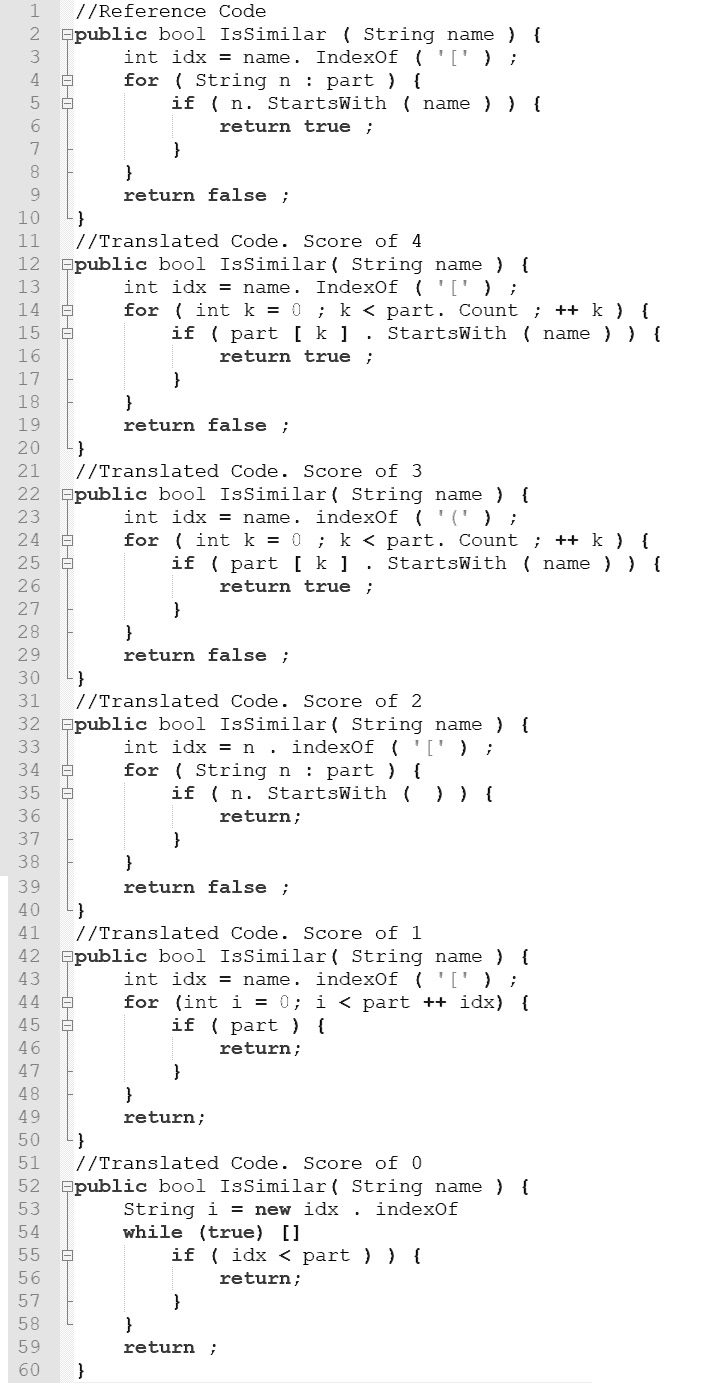
\includegraphics{scoreExamples}

We conducted the same human study for the translated results from all above models with a total of 2,250 manual assignments of such scores. Let us call them \textbf{{\em
    semantic scores}}.


%of both lpSMT and
%mppSMT models. As a result, we have scores for 375 pairs of methods
%for each model. From now on, we regard those scores as \textbf{{\em
%    Semantic score}}.

%\begin{figure}
%\caption{Scoring Examples}
%\centering
%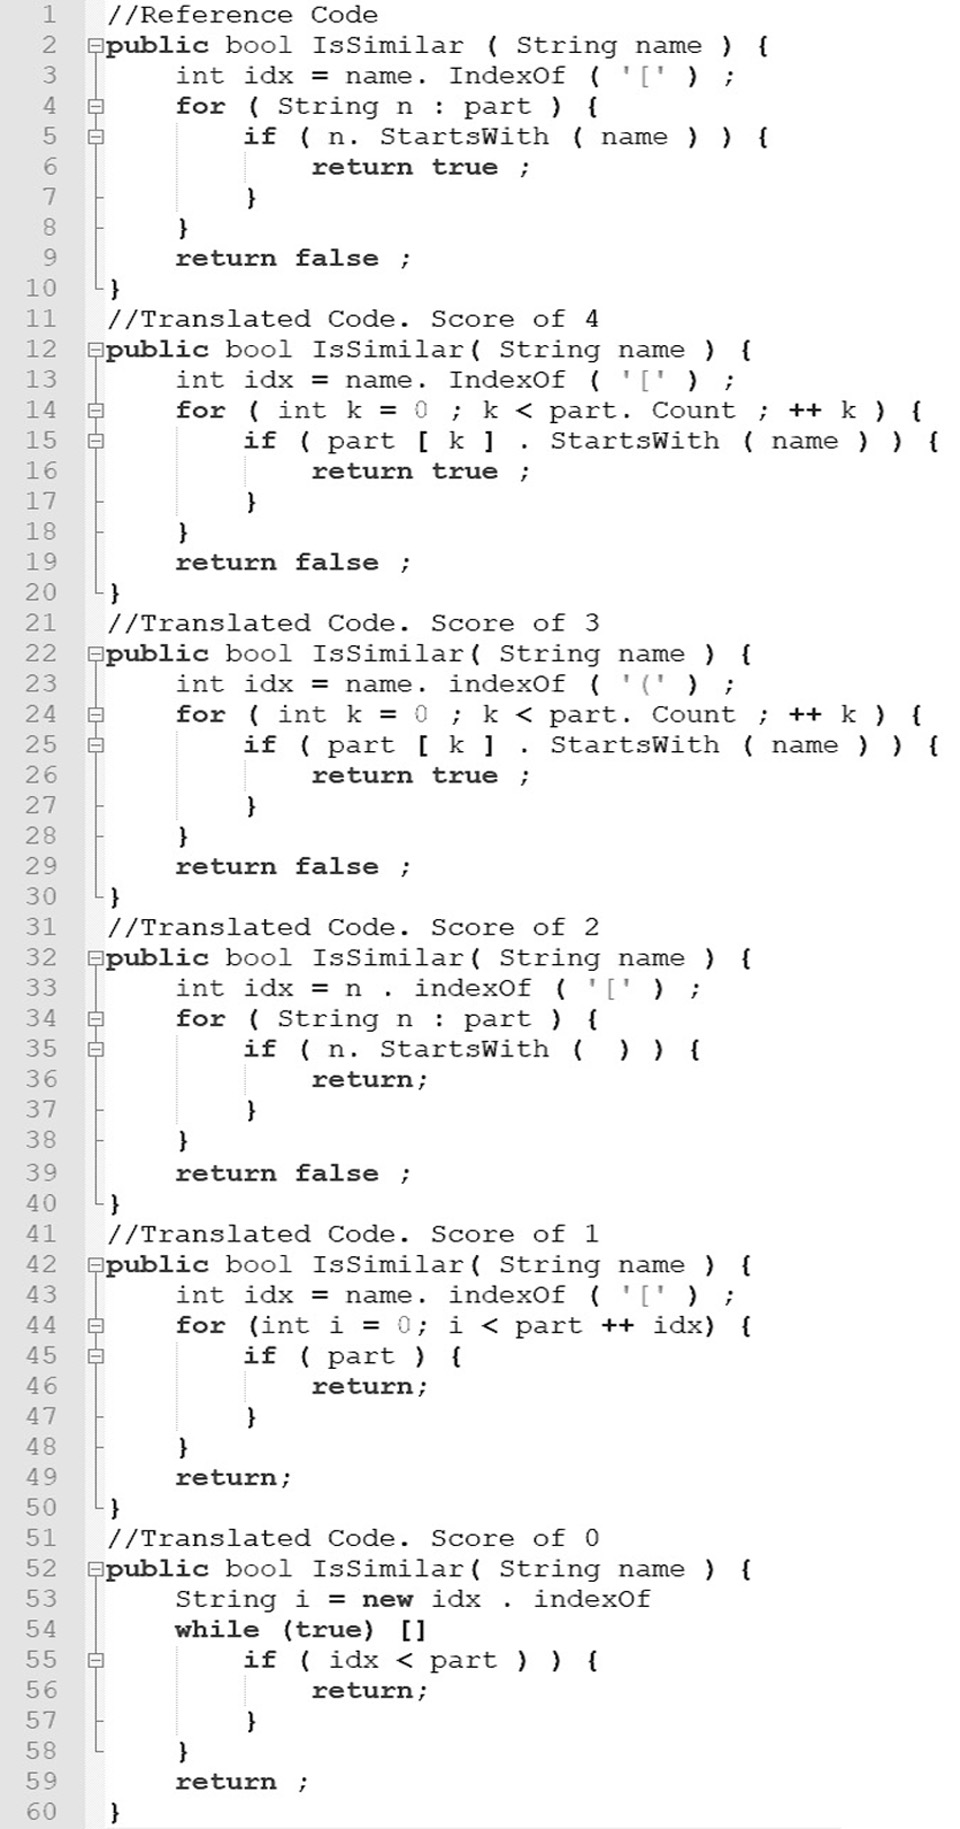
\includegraphics{img/scoreExamples}
%\label{fig:scoreEG}
%\end{figure}


%Our hypothesis states that \emph{\textit{BLEU score does not measure well the similarity in term of semantics between the reference and migrated source code}}. Therefore, given a pair of methods (reference one and machine translated one), we need a metric that can measure the similarity in term of semantics between them. As we know of, there is no automated metrics to do that task. To determine semantic similarity score, we used a human subject to manually evaluate pairs of methods to see how close they are in term of semantic/functionality. Specifically, scoring is done based on the human effort to fix the translated method to achieve the same functionality as of the reference one. The detailed scoring guidelines are presented in Table\ref{table:criteria}. The human subject is a senior developer who is fluent in both Java and C\#. He was given a pair of methods in C\# (machine generated one and reference one), the original method in Java, and the context project from which the methods come from. Then, he was told to evaluate pairs of methods in C\#, and give score as our guideline above and table \ref{table:criteria}. He could also refer back to the original Java method and project for a better understanding of the context. Below are examples for each score from -2 to 2:\\
%To determine semantic similarity score between pair of methods, we manually scored each pair from 0 to 6 based on the human effort to fix a translated method to a referenced one. Specifically, we list the criteria to score in Table  with a score of 0 means the pair of methods are totally different, and a score of 6 means they are totally the same. Scoring also follows the following principles: 1. An effort to fix a syntactical error (misplacing a semi-colon, parenthesis...) has less weight than an effort to fix a semantical error (wrong branch, wrong function call...). 2. A fix that requires adding sources code has more weight than one that requires removing/replacing. 3. A fix for user-defined program elements (identifier, simple name, method name) is more 'pricey' than a fix for keyword (this, if, for...). Example (of scores 1,3,5).

%Since our dataset contains a large number of pairs of methods, it would take a lot of efforts to manually evaluate all of them. Hence, we took a sample from our population of total 34,209 pairs. According to \cite{website}, our sample size is 375 with confidence level of $95\%$ and margin of error $5\%$. After we conducted the human experiment with 375 pairs of methods, we normalized the result on 0-1 range with 0 is respected to -2 and 1 is respected to 2.



\section{Empirical Results}
\label{sec:bleuresult}

In this section, we present the empirical results to validate our hypothesis that 
\textit{BLEU is not effective in evaluating translation quality of source code migration task}
\subsection{Correlation between BLEU and Semantic scores}
To justify the first part of our hypothesis, BLEU score does not reflect well 
the semantic accuracy of results translated by a particular model, 
we show the relation between BLEU scores and human judgments via semantic scores. 
We use Pearson's correlation coefficient~\cite{PearsonCorrelation} to gauge
how strong their relation is. The correlation coefficient has value
between -1 and 1, where 1 indicates the strongest positive relation, -1
indicates the strongest negative relation, and 0 indicates no relation.

Figures~\ref{fig:BleuSemlpSMT} and~\ref{fig:BleuSemMppSMT} show the
scatter plots between two metrics: BLEU and Semantic. Each point
represents the scores of a pair of methods where its $x$-axis value is
for BLEU scores and $y$-axis value is for semantic scores. The
correlation coefficient between BLEU and semantic scores for the model
mppSMT is 0.523 and for the model lpSMT is 0.570. These possitive values 
are closer to 0.5 than to 1.0. This means there is a positive but weak 
relationship between BLEU score and semantic score. The weak correlations %help me to check grammar
between the metrics on the results translated by lpSMT and mppSMT are 
demonstrated in figures~\ref{fig:BleuSemlpSMT} and~\ref{fig:BleuSemMppSMT}.

%\emph{Observation 1:} 
In figure ~\ref{fig:BleuSemlpSMT}, for many specific values of BLEU, it 
is clear that associated semantic scores can be in a wide range. For 
instance, the BLEU score of 0.75, the associated semantic scores are 
from 0.25 to 1 \textbf{Ngoc: can u mark in the figure please}. Thus, from this 
observation, we conclude that the results migrated by certain models 
with high BLEU scores might not archive high semantic scores. 
%There are two reasons for this. 
%

In our sample set, these results can fall in two main cases. 
First, the translated methods might have multiple correct phrases, but in the 
incorrect order, those method can be incorrect, even incompliable.
%useless and justified as so in human judgment.
%
For example, in Figure~\ref{fig:issueexample2}, the translated method
misplaces the position of the bracelet which makes the method has low
Semantic score, but high BLEU score. 
%
%Another reason for this implication is that resulting method does not capture the important
%program elements. 
In other case, the migrated results are incomplete methods missing elements
that are trivial for the translation model, but this violate syntactic rules 
of the target language. For example, the result contains mostly keywords and
punctuation such as \code{if}, \code{public}, \code{()}, but misses
out the important program elements such as function calls or variable
names. In this case, it will have low semantic score while having
a moderate to high BLEU score. These cases indicate the weakness of BLEU metric 
in evaluating the translated results in programing language where syntaxes are well defined.

%\emph{Observation 2:} For a fixed value of Semantic score, there can
%be many associated BLEU values. Specifically, in the model lpSMT, with
%a Semantic Score of 1, the BLEU scores can vary greatly between 0-1,
%which is reflected on the top horizontal line of dots in the
%Figure~\ref{fig:BleuSemlpSMT}. Similarly, in
%Figure~\ref{fig:BleuSemMppSMT}, with the Semantic Score of 1, the BLEU
%scores are in the range of 0.5 to 1.
For the results translated by mppSMT (figure \ref{fig:BleuSemMppSMT}), 
for a particular value of  semantic score, there can be many associated 
BLEU values that spread out over a wide range. Specifically, in the model 
mppSMT, with the absolute semantic score, the BLEU scores can vary greatly 
between 0.5-1. By this empirical results, it can be concluded that for 
some models, the method achieving higher semantic score does not necessarily 
have higher BLEU score. 

%From this observation, it can be implied that translated code can have
%low BLEU score, but high Semantic score. This can be explained by two
%reasons. 
From our sample data, we observe that there are two main reasons leading 
to this phenomenon.
%
First, a translated method can use different code structure from the 
reference one to perform the same functionality. Figure \ref{?} shows an example
that got maximum semantic score, but has low BLEU score (0.4). In this example, 
the translated method uses a \code{for} loop instead of a \code{foreach} 
loop as in the reference code. The second reason causing this phenomenon 
is that the whitespace issue. For example, in figure \ref{?}, the translated method has the 
tokens \code{changeMe()}, but the reference method has \code{changeMe ()}. The former 
is interpreted as one token while the former is interpreted as two tokens. 
This situation reduces the precision on phrases, but the human subject still
evaluated the result with high semantic score. By this experiment, we also empirically 
verify the argument that the forcusing on the lexical precision of BLEU makes
this metric is not able to capture other aspects such as dependencies 
that contribute to the sementics of source code.

%TODO need to verify
In conclusion, BLEU does not reflect well the
semantics of source code, and it is not suitable to use in evaluating
semantic accuracy of a SMT-based code migration system.

\subsection{The Use of BLEU in Comparing Models}
To validate the use of BLEU in comparing different SMT-based code migration systems, we conduct study to see if the change in BLEU scores over models reflect the change in translation quality represented by human judgments of Semantic score. For a same set of 375 original Java methods, the two models GNMT and mppSMT generates two sets of 375 translated methods. Each set has its own BLEU scores and Semantic scores. We ignored pairs of translated results if they have the same BLEU score or Semantic score (136 of the cases). For the remaining results, we found out that in \textbf{34\%} of the cases, the change in BLEU score contradicts the change in Semantic score. It means an improvement in BLEU score leads to a decrease in Semantic score and vice versa. In other words, if one function is translated by two migration models, one-third of the time, the result which has higher BLEU score actually has lower translation quality than the other. Consequently, BLEU is not reliable to use in comparing different SMT-based migration models. 

\begin{figure}
\caption{BLEU metric vs Semantic metric (lpSMT model)}
\centering
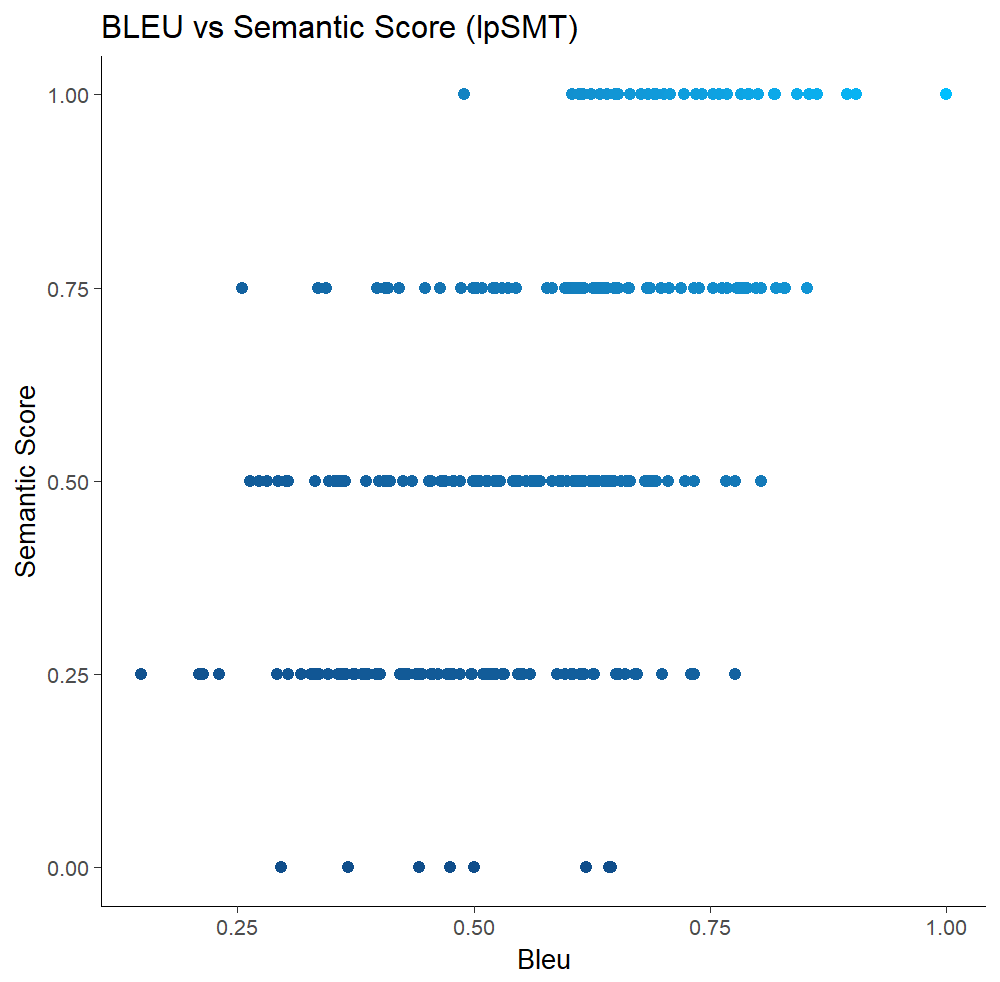
\includegraphics{img/bleuvssemantic_lpSMT.png}
\label{fig:BleuSemlpSMT}
\end{figure}

\begin{figure}
\caption{BLEU metric vs Semantic metric (mppSMT model)}
\centering
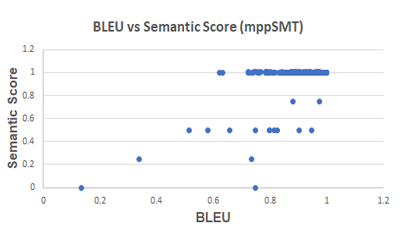
\includegraphics{img/bleuvssemantic_mppSMT.png}
\label{fig:BleuSemMppSMT}
\end{figure}


\section{Proposal}
\subsection{\model}
%For a SMT-based migration system, BLEU has always been like this... doing that....

%From the results in section 5, BLEU did not reflect the semantic accuracy of source code. --> We need a better metrics to replace BLEU

%Needed metric should be 
%Reflect semantical meaning of sources code.
%Automated
%Low computation's cost
%Independent of programming language
%Independent of MT model's type

Considering all those requirements above, we introduce {\model}, a novel automated metric that can reflect semantic accuracy of translated code. {\model} is also independent of programming languages and machine translation models used in migration system. {\model} measures the semantic accuracy of the resulting code by comparing the program dependence graph (PDG) between them. PDG captures both the data and control dependencies among program entities. Because of its properties, we expect PDG can represent well the semantic level of source code. To reduce the high computational cost, we vectorize the PDG and calculate the vector difference to estimate the graph difference. This way, we would make sure that our model is practical and applicable in large scaled systems. 

When applying MT on source code, there always exists the problem that the translated code is not compilable. Thus, it is impossible to build PDG on those code. To cope with the problem, our model is designed as best-effort, layered metric  : If the translated code can be built into PDG, we calculate {\model} in term of graph difference. If the translated code cannot be built into PDG but is compilable, we calculate {\model} in term of syntax tree edit distance. If the translated code is not compilable, we calculate {\model} in term of string edit distance. 

if (GVED(s,t) != -1) RUBY(s,t) = GVED(s,t)\\
else if (TREED(s,t) != -1) RUBY(s,t) = TREED(s,t)\\
else RUBY(s,t) = SED(s,t)
\section{Related Work}

There exist
many studies aiming to measure the functionality similarity of source
code, which utilize the similarities of structures and
dependencies~\cite{clone-tse07,roy09,baker97,ccfinder,cpminer,deckard,deckard2,horwitz01}.
%baxter98,ducasse99
However, they are not reliable as their results sometimes contradict
with human judgments on semantic accuracy~\cite{deckard2}.

However, there exists criticism on BLEU
as Callison-Burch {\em et al.}~\cite{Callison} argued that an
improvement in BLEU metric is not sufficient nor necessary to show an
improvement in translation quality. Despite such criticism,

\section{Conclusion}

% (36.8\% relatively higher). 
%We also built an Eclipse plugin that automatically adds the import
%statements of the required libraries for a given code snippet and sets
%up the Maven links to the repositories for those libraries.

%\section*{Acknowledgments}
%We would like to thank 
%Sarah Nadi,
%Stas Negara,
%Mihai Codoban,
%Sruti Srinivasa, % Sruti did not give feedback as she was busy with her own CHI submissions
%Zhen Yu,
%Ameya Ketkar,
%and Samantha Khairunnesa 
%for providing valuable feedback on earlier drafts of this paper.

% TODO: add here the Grant numbers

\newpage

\balance
%\bibliographystyle{abbrv}
%\citestyle{acmauthoryear}

\bibliographystyle{ACM-Reference-Format}

\setcitestyle{numbers,sort&compress}

%\setcitestyle{numbers,sort&compress}
\bibliography{fse18}



% That's all folks!
\end{document}
